\chapter{Proof of concept}

\section{Componentkeuze}

\begin{figure}[!htbp]
    \includesvg[width=\textwidth]{./graphics/4-Oplossing_totaal.svg}
    \caption[short description]{elaborate description}
    \label{fig:Componentkeuze}
\end{figure}

\subsection{XCP-ng}

\subsection{Xen Orchestra}

\subsection{Ubuntu Server}
Gezien SmartEye momenteel zelf gebruiker is van Ubuntu Server voor hun serverinfrastructuur, lag deze keuze voor de hand. Deze open-source Linux-distributie is bovendien gratis en wordt ondersteund door een goede communitywerking.

\subsection{OPNsense}
OPNsense is een fork van pfSense. Grootste verschillen tussen beide zijn voornamelijk de frequentie van updates (OPNsense komt met meer kleine updates terwijl pfSense opteert voor minder, maar grotere updates) en meer overzichtelijke user interface van OPNsense. Ook heeft OPNsense een actievere community.

\subsection{nProbe}

\subsection{ntopng}

\subsection{Python}

\section{Implementatie \& configuratie}
\subsection{Algemene systeemconfiguratie}
Belangrijk bij het werken met logs is dat deze consistent zijn over alle servers en netwerkdevices heen. Zo moeten deze allemaal hetzelfde tijdssysteem hanteren zodat na het consolideren van logs het onmiddellijk en probleemloos mogelijk is om alle alerts eenduidig op een tijdslijn te plaatsen zodat tijd gerelateerde analyse mogelijk is.

\paragraph{}
Niet alleen moeten alle servers hetzelfde tijdssysteem hanteren, ook mag de problematiek van winteruur en zomeruur geen spelbreker zijn door overlap of gaten in de tijdslijn te creëren.

\paragraph{}
Om de hierboven geschetste problemen te voorkomen, hebben we geopteerd voor het gebruik van Cloudflare Time Services. Hierbij wordt NTP (Network Time Protocol) gebruikt om tijd te synchroniseren tussen servers en netwerkdevices. Cloudflare beschikt hiervoor over een anycast-netwerk van 330 locaties.

\subsection{Firewall configuratie}

\paragraph{Configuratie van de NetFlow-export naar nProbe}
Onderstaande screenshot geeft de NetFlow exporter-configuratie weer.
We luisteren zowel op LAN als WAN interfaces omdat we zoveel mogelijk trafiek willen kunnen monitoren.

\paragraph{}
Bij de configuratie kunnen we opteren om gebruik te maken van NetFlow versie 5 of versie 9. We opteerden voor versie 9. Deze versie is template gebaseerd en bijgevolg meer flexibel en uitbreidbaar. Bovendien ondersteunt versie 9 IPv6.

\paragraph{}
Het veld ‘destination’ bevat het IP van de nProbe flowcollector waarheen we alle flow data willen sturen.

\paragraph{}
Een flow blijft ‘actief’ zolang er berichten worden aan toegevoegd. Na 30 seconden wordt een flow echter steeds afgesloten en doorgestuurd. Bijgevolg kan het zijn dat niet alle berichten in eenzelfde flow opgenomen werden. De reden van deze ingestelde time-out is echter om het feit op te vangen dat zolang een flow open is, de berichten in deze flow ook nergens zichtbaar zijn voor analyse.

\paragraph{}
Als een flow 10 seconden geen nieuwe berichten ontvangen heeft, wordt deze ook afgesloten en doorgestuurd. Dit is bijvoorbeeld van belang bij UDP dat stateless is.

\begin{figure}[!htbp]
    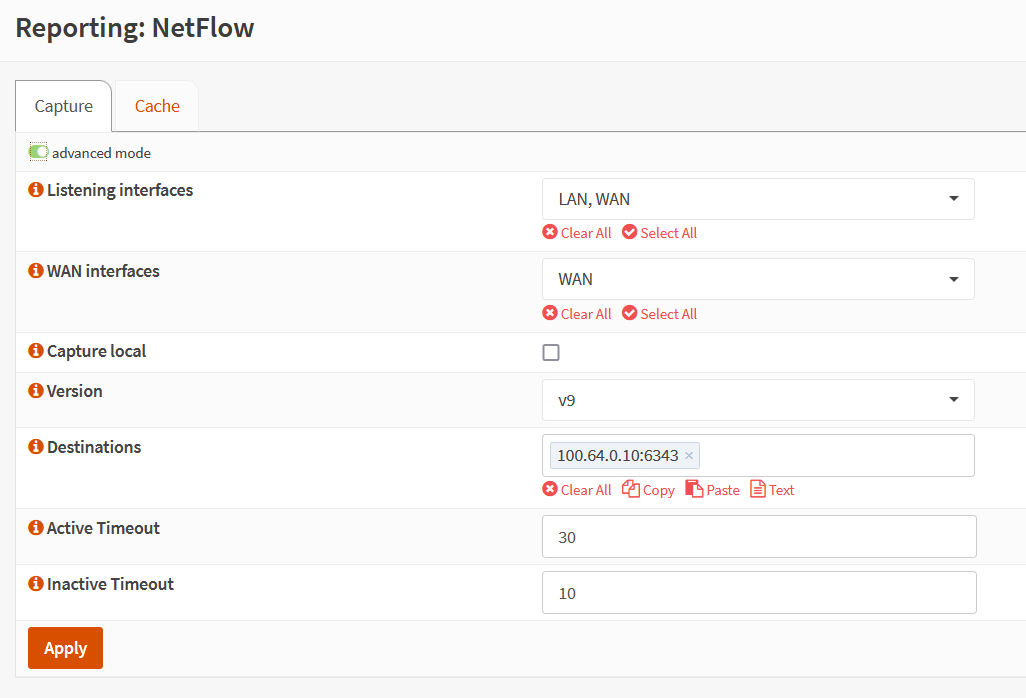
\includegraphics[width=\textwidth]{./graphics/opnsense_netflow_conf.PNG}
    \caption[OPNsense NetFlow configuratie]{elaborate description}
    \label{fig:FirewallNetflow}
\end{figure}

\paragraph{Het aanpassen van de ephemeral port range van de firewall}
De OPNsense firewall draait onderliggend FreeBSD. In onderstaande screenshot geven we aan welke port range de firewall voor zijn eigen werking mag gebruiken. De Carrier-Grade NAT moet immers deterministisch zijn. Alle combinaties ‘IP + port’ moeten bijgevolg uniek gebruikt worden. Zo mogen niet alleen tenants geen combinaties dubbel gebruiken, maar ook de firewall mag geen combinaties gebruiken die door een tenant gebruikt worden. Hiertoe geven we de firewall zijn eigen port range.

\begin{figure}[!htbp]
    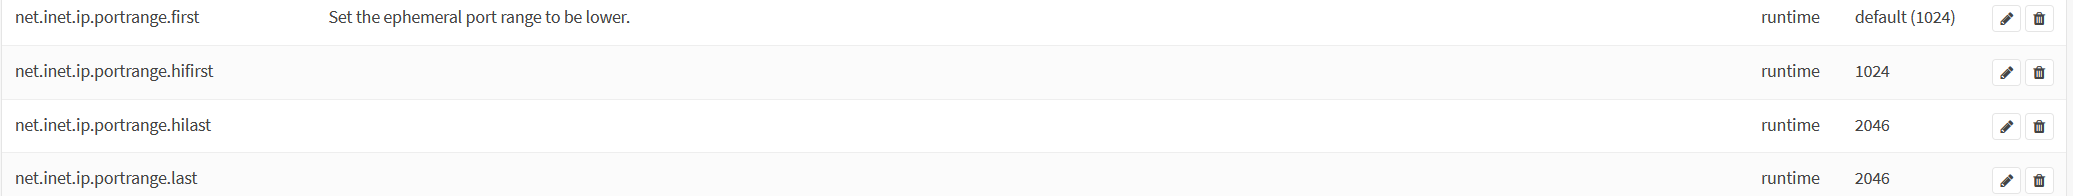
\includegraphics[width=\textwidth]{graphics/opnsense_tunables_portrange.PNG}
    \caption[OPNsense tunables portrange]{elaborate description}
    \label{fig:FirewallTunables}
\end{figure}

\paragraph{Het aanmaken van de Carrier-Grade NAT-rules op de firewall via de API}
Onderstaande screenshot geeft alle Carrier-Grade NAT rules weer die op de firewall werden geïmplementeerd. Deze rules werden opgebouwd met behulp van een Python script.

\begin{figure}[!htbp]
    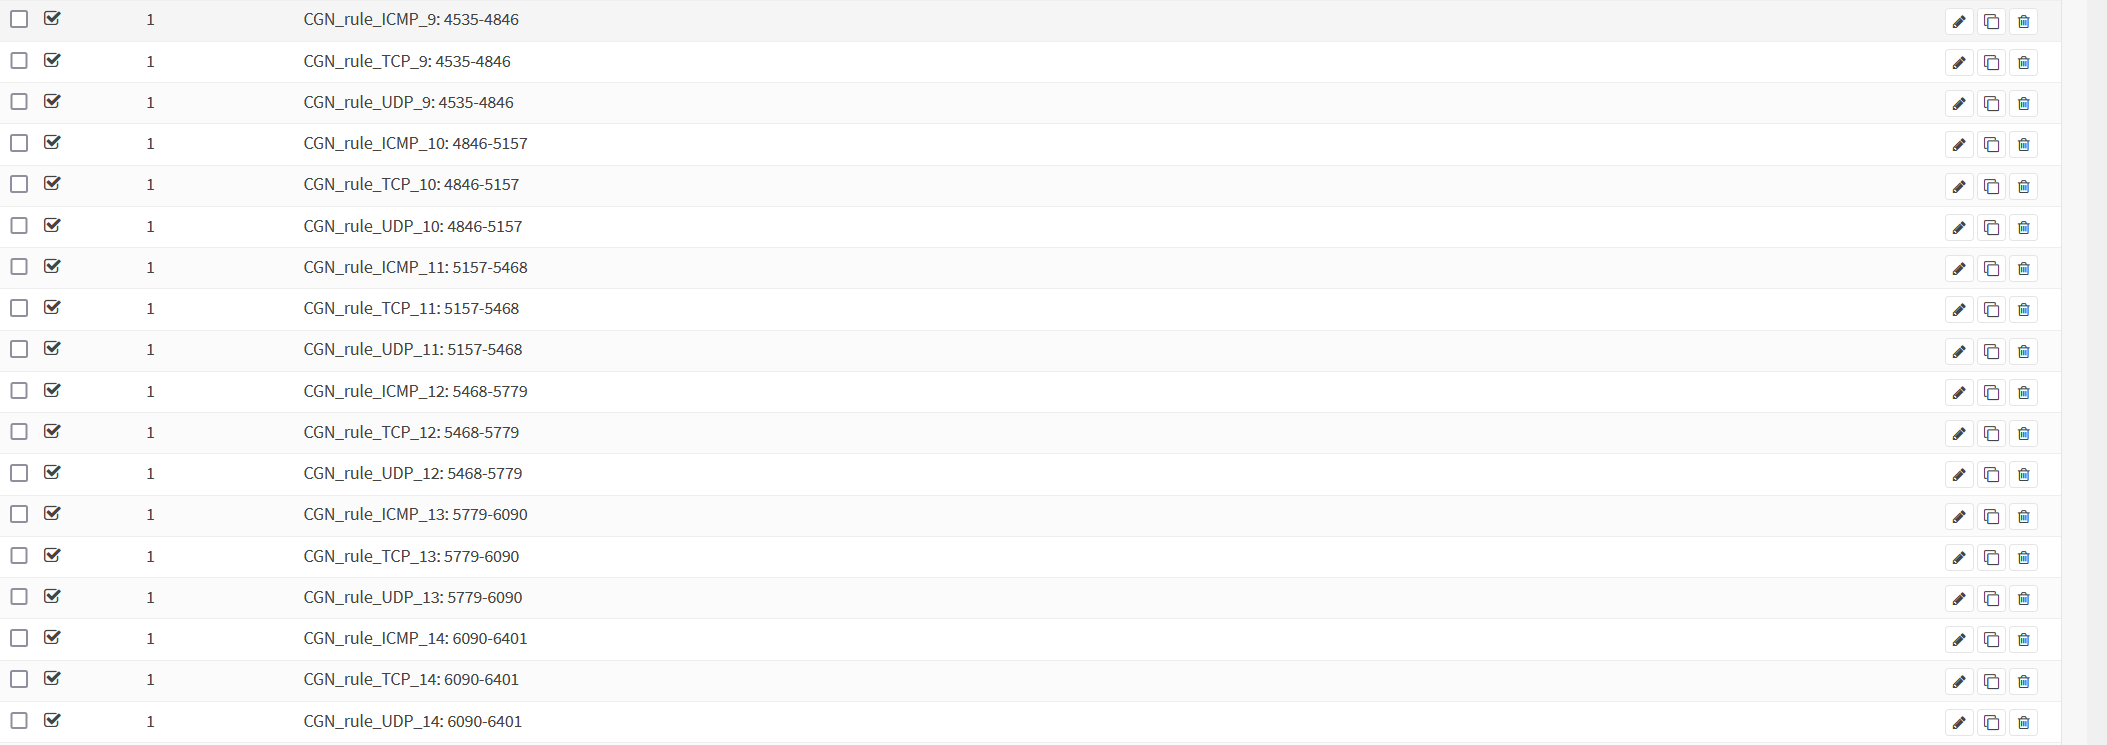
\includegraphics[width=\textwidth]{graphics/opnsense_cgnat_rules.PNG}
    \caption[OPNsense met CGN regels]{elaborate description}
    \label{fig:FirewallCGNRules}
\end{figure}

Het Python script dat hierna wordt weergegeven, genereert alle vereiste rules. In totaal zijn dit er snel enorm veel, namelijk het aantal tenants maal 3, gezien elke rule moet gelden voor zowel ICMP, UDP als TCP.

\paragraph{}
Het script bevat volgende variabelen:

\begin{itemize}
    \item Het aantal beschikbare poorten, namelijk $2^{16}$.
    \item De gereserveerde (en dus niet bruikbare) systeempoorten 0 t/m 1023.
    \item De port range die door de firewall zelf gebruikt wordt.
    \item Het aantal tenants dat dient geconnecteerd te worden.
\end{itemize}

Op basis van deze informatie berekent het script hoeveel poorten er maximaal per tenant kunnen worden toegewezen.
Vervolgens gaat het script aan elke tenant een range toekennen.
Per range worden dan drie API calls richting de firewall gelanceerd om voor zo voor elke range een ICMP, UDP en TCP source NAT rule aan te maken.

\begin{minted}{python}
    import json
    import os

    import dotenv
    import requests
    import urllib3

    urllib3.disable_warnings()

    dotenv.load_dotenv('credentials.env')
    credentials = {'key': os.environ['API_KEY'], 'secret': os.environ['API_SECRET'],
        'base_url': os.environ['API_BASE_URL']}

    total_amount_ports = (2 ** 16) - 1
    system_ports = 1023
    firewall_ports = 1023
    amount_of_CPEs = 204


    def create_url(module, controller, command, base_url=credentials['base_url'], parameters=''):
    url = f'{base_url}/{module}/{controller}/{command}/{parameters}'

    return url


    def api_call(url, request_method, verify=False, auth=(credentials['key'], credentials['secret']), json=None):
    if request_method == 'POST':
    if json:
    r = requests.post(url=url, verify=verify, auth=auth, json=json)

    else:
    r = requests.post(url=url, verify=verify, auth=auth)

    elif request_method == 'GET':
    r = requests.get(url=url, verify=verify, auth=auth)

    return r


    def get_amount_cgn_ips(ports_per_CPE, total_amount_ports=total_amount_ports, system_ports=system_ports,
    firewall_ports=firewall_ports):
    port_range_list = []

    for index, port_range in enumerate(range(system_ports + firewall_ports + 1, total_amount_ports + 1, ports_per_CPE)):
    port_range_end = port_range + ports_per_CPE

    if port_range_end < total_amount_ports:
    port_range_list.append(f'{port_range}-{port_range_end}')

    cgn_ip_count = len(port_range_list)

    return cgn_ip_count, port_range_list


    def get_amount_ports_cpe(amount_of_CPEs):
    ports_per_CPE = (total_amount_ports - (system_ports + firewall_ports)) // amount_of_CPEs
    return get_amount_cgn_ips(ports_per_CPE)


    ports = get_amount_ports_cpe(amount_of_CPEs)

    s = api_call(create_url(module='firewall', controller='filter', command='savepoint'), 'POST')
    savepoint = json.loads(s.text)['revision']
    print(f'{s.status_code}\n{s.text}')

    for index, port_range in enumerate(ports[1]):
    first_octet = 100
    second_octet = 64 + ((index + 1) // 255 ** 2)
    third_octet = (index + 1) // 255
    last_octet = (index + 1) % 255

    _, port_range_last = port_range.split("-")

    if int(port_range_last) < total_amount_ports and second_octet <= 127:
    data = {
        "rule": {
            "interface": "wan",
            "source_net": f"{first_octet}.{second_octet}.{third_octet}.{last_octet}/32",
            "target": "wanip",
            "categories": "ae1d4052-c3b4-4e21-b8f6-f7962a4b18ef"
        }
    }
    data["rule"]["protocol"] = "ICMP"
    data["rule"]["description"] = f"CGN_rule_ICMP_{index + 1}: {port_range}"
    r = api_call(create_url(module='firewall', controller='source_nat', command='addRule'), 'POST', json=data)
    print(f'{r.status_code}\n{r.text}')

    data["rule"]["protocol"] = "TCP"
    data["rule"]["description"] = f"CGN_rule_TCP_{index + 1}: {port_range}"
    data["rule"]["target_port"] = f"{port_range}"
    r = api_call(create_url(module='firewall', controller='source_nat', command='addRule'), 'POST', json=data)
    print(f'{r.status_code}\n{r.text}')

    data["rule"]["protocol"] = "UDP"
    data["rule"]["description"] = f"CGN_rule_UDP_{index + 1}: {port_range}"
    data["rule"]["target_port"] = f"{port_range}"
    r = api_call(create_url(module='firewall', controller='source_nat', command='addRule'), 'POST', json=data)
    print(f'{r.status_code}\n{r.text}')

    s = api_call(create_url(module='firewall', controller='filter', command='apply', parameters=savepoint), 'POST')
    print(f'{s.status_code}\n{s.text}')

    s = api_call(create_url(module='firewall', controller='filter', command='cancelRollback', parameters=savepoint), 'POST')
    print(f'{s.status_code}\n{s.text}')
\end{minted}
\begin{listing}[!htbp]
    \caption[Python CGN code]{elaborate description}
    \label{code:PythonCGN}
\end{listing}

\subsection{nProbe}
\begin{listing}[!htbp]
    \caption[nProbe configuration]{elaborate description}
    \label{code:nProbeConf}

    \begin{minted}{bash}
        --collector-port=6343
        --ntopng=zmq://100.64.0.11:5556
        --zmq-probe-mode
        -T="@NTOPNG@"
    \end{minted}
\end{listing}

\subsection{ntopng}
\begin{listing}[!htbp]
    \caption[ntopng configuration]{elaborate description}
    \label{code:ntopngConf}

    \begin{minted}{bash}
        --interface=tcp://*:5556c
        --https-port=3001
        --http-port=0
        --local-networks=100.64.0.0/10
    \end{minted}
\end{listing}

\section{Test}
We willen met deze test verdachte activiteit door een tenant simuleren. We doen dit door het draaien een nmap scan naar een adres dat aan de andere kant van de firewall gelegen is vanop de (arbitrair gekozen) server met IP 100.64.0.11 en port range 5157 - 5468, waar in dit geval ook ntopng op draait. Bij deze opzet werd het IP statisch toegekend.

\subsection{Carrier-Grade NAT’ing}
Onderstaande output is het resultaat een ‘sudo nmap -p- 192.168.10.1’. Op deze screenshot zien we dat de NAT’ing effectief gebeurt op de firewall.

\begin{figure}[H]
    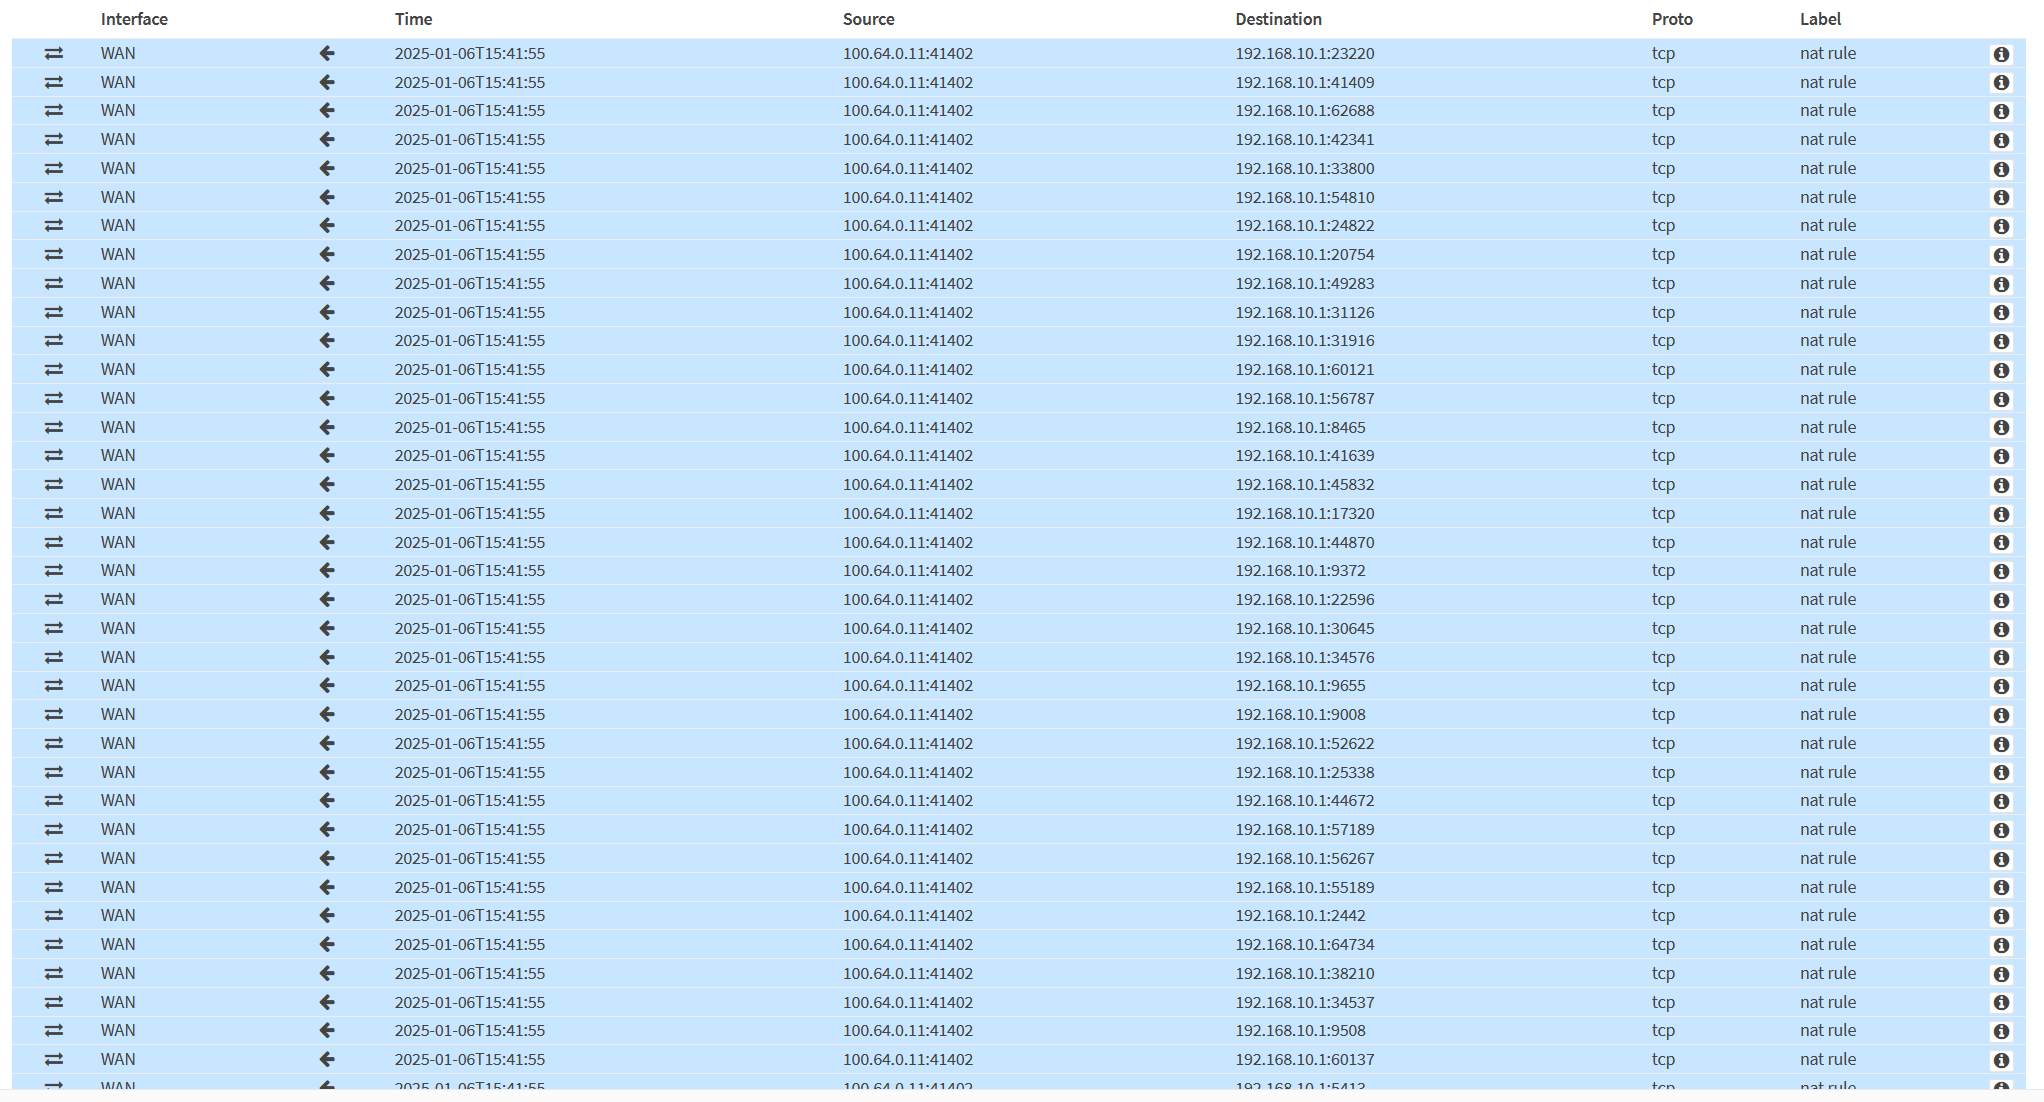
\includegraphics[width=\textwidth]{graphics/nmap_nat_table.PNG}
    \caption[OPNsense CGN regels in werking deel 1]{elaborate description}
    \label{fig:FirewallGCNWorksA}
\end{figure}

\subsection{Resultaat Carrier-Grade NAT’ing}
Onderstaande screenshot geeft de doorgelaten ge-NAT’te trafiek weer. Bemerk dat alle trafiek zich (zoals gedefinieerd en dus verwacht) binnen de source port range 5157 – 5468 bevindt.

\begin{figure}[H]
    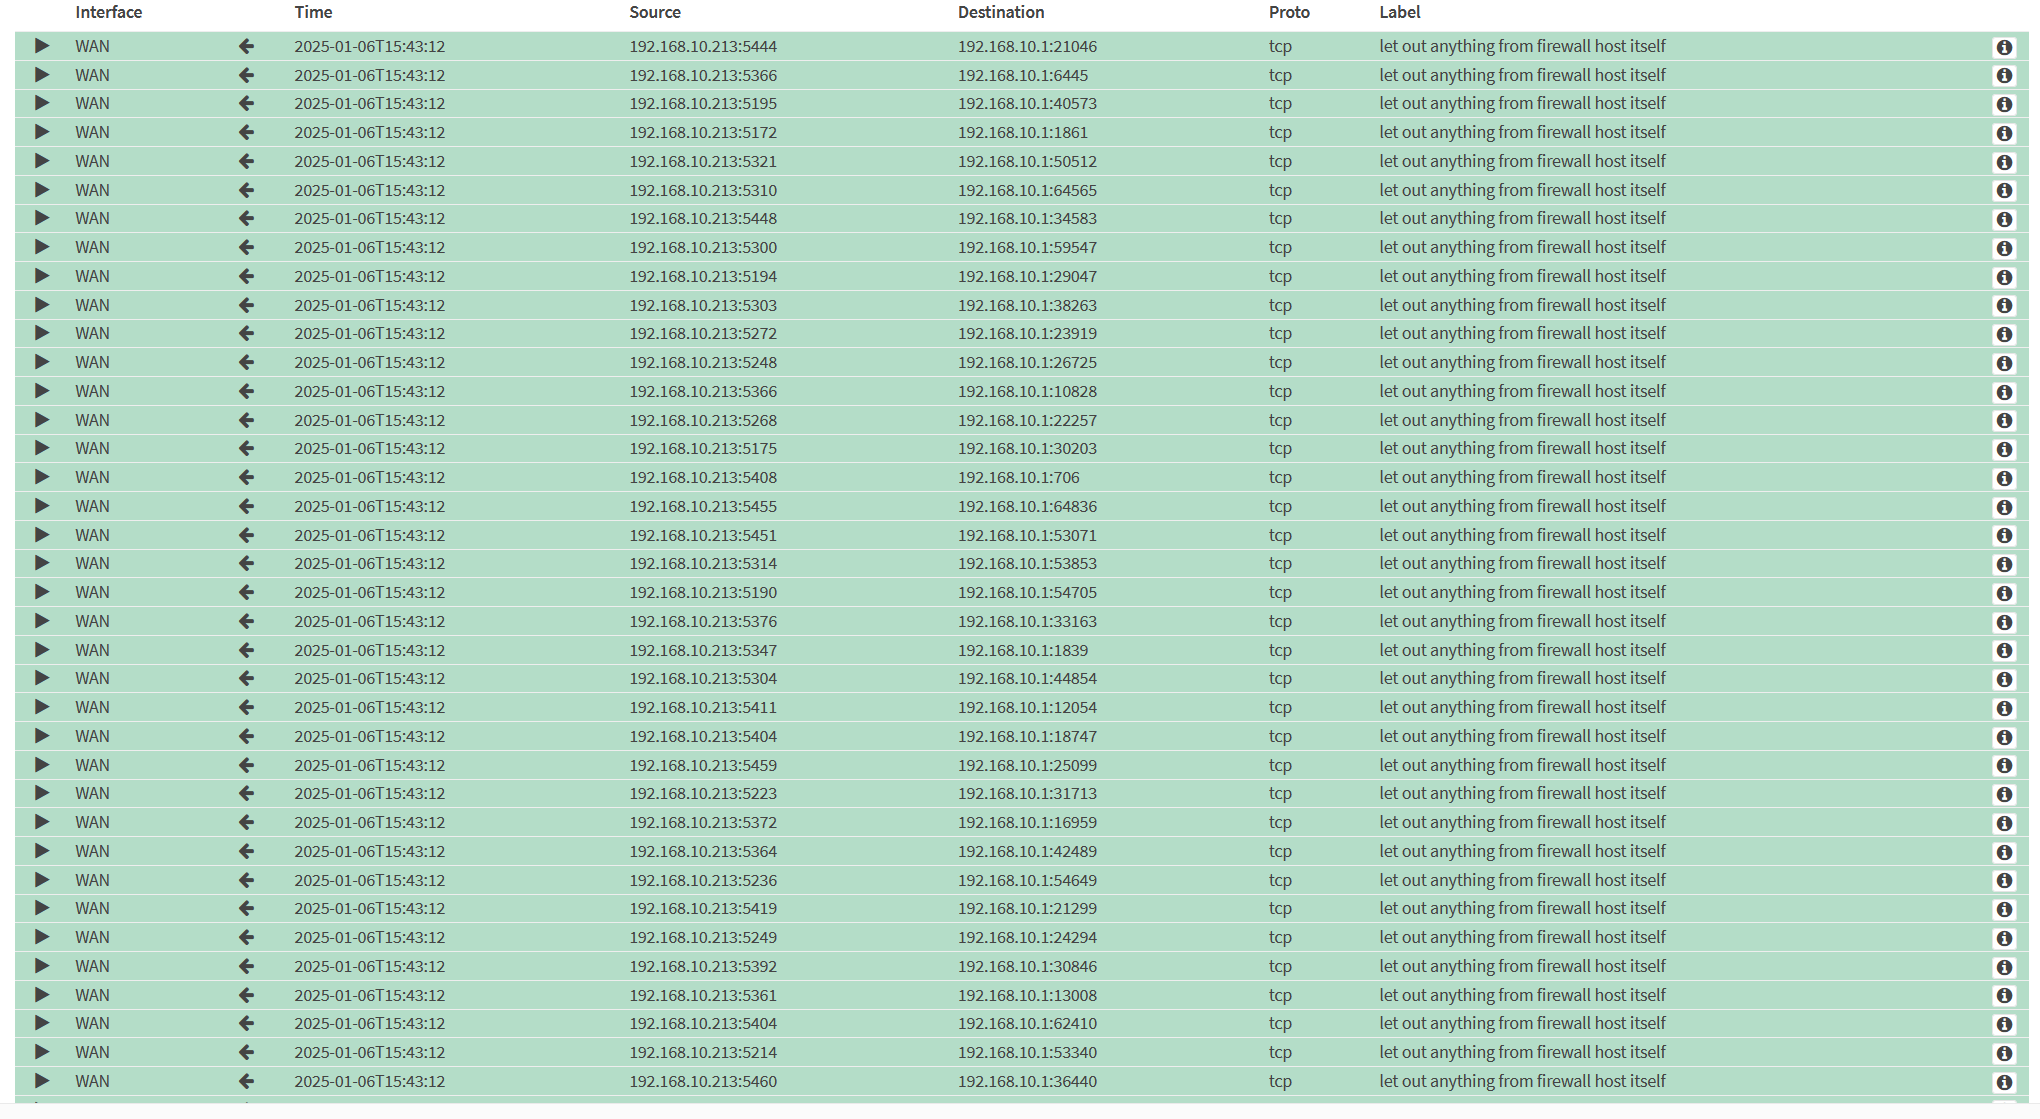
\includegraphics[width=\textwidth]{graphics/nmap_firewall_table.PNG}
    \caption[OPNsense CGN regels in werking deel 2]{elaborate description}
    \label{fig:FirewallGCNWorksB}
\end{figure}

\subsection{Geëxporteerde flows komen binnen op ntopgn}
De doorgelaten ge-NAT’te trafiek binnen de source port range 5157 – 5468 wordt door de firewall geëxporteerd naar de nProbe flowcollector die de data formatteert en vervolgens naar de ntopng flow analyser doorstuurt. Op ntopng resulteert dit in onderstaande screenshot.

\begin{figure}[htb]
    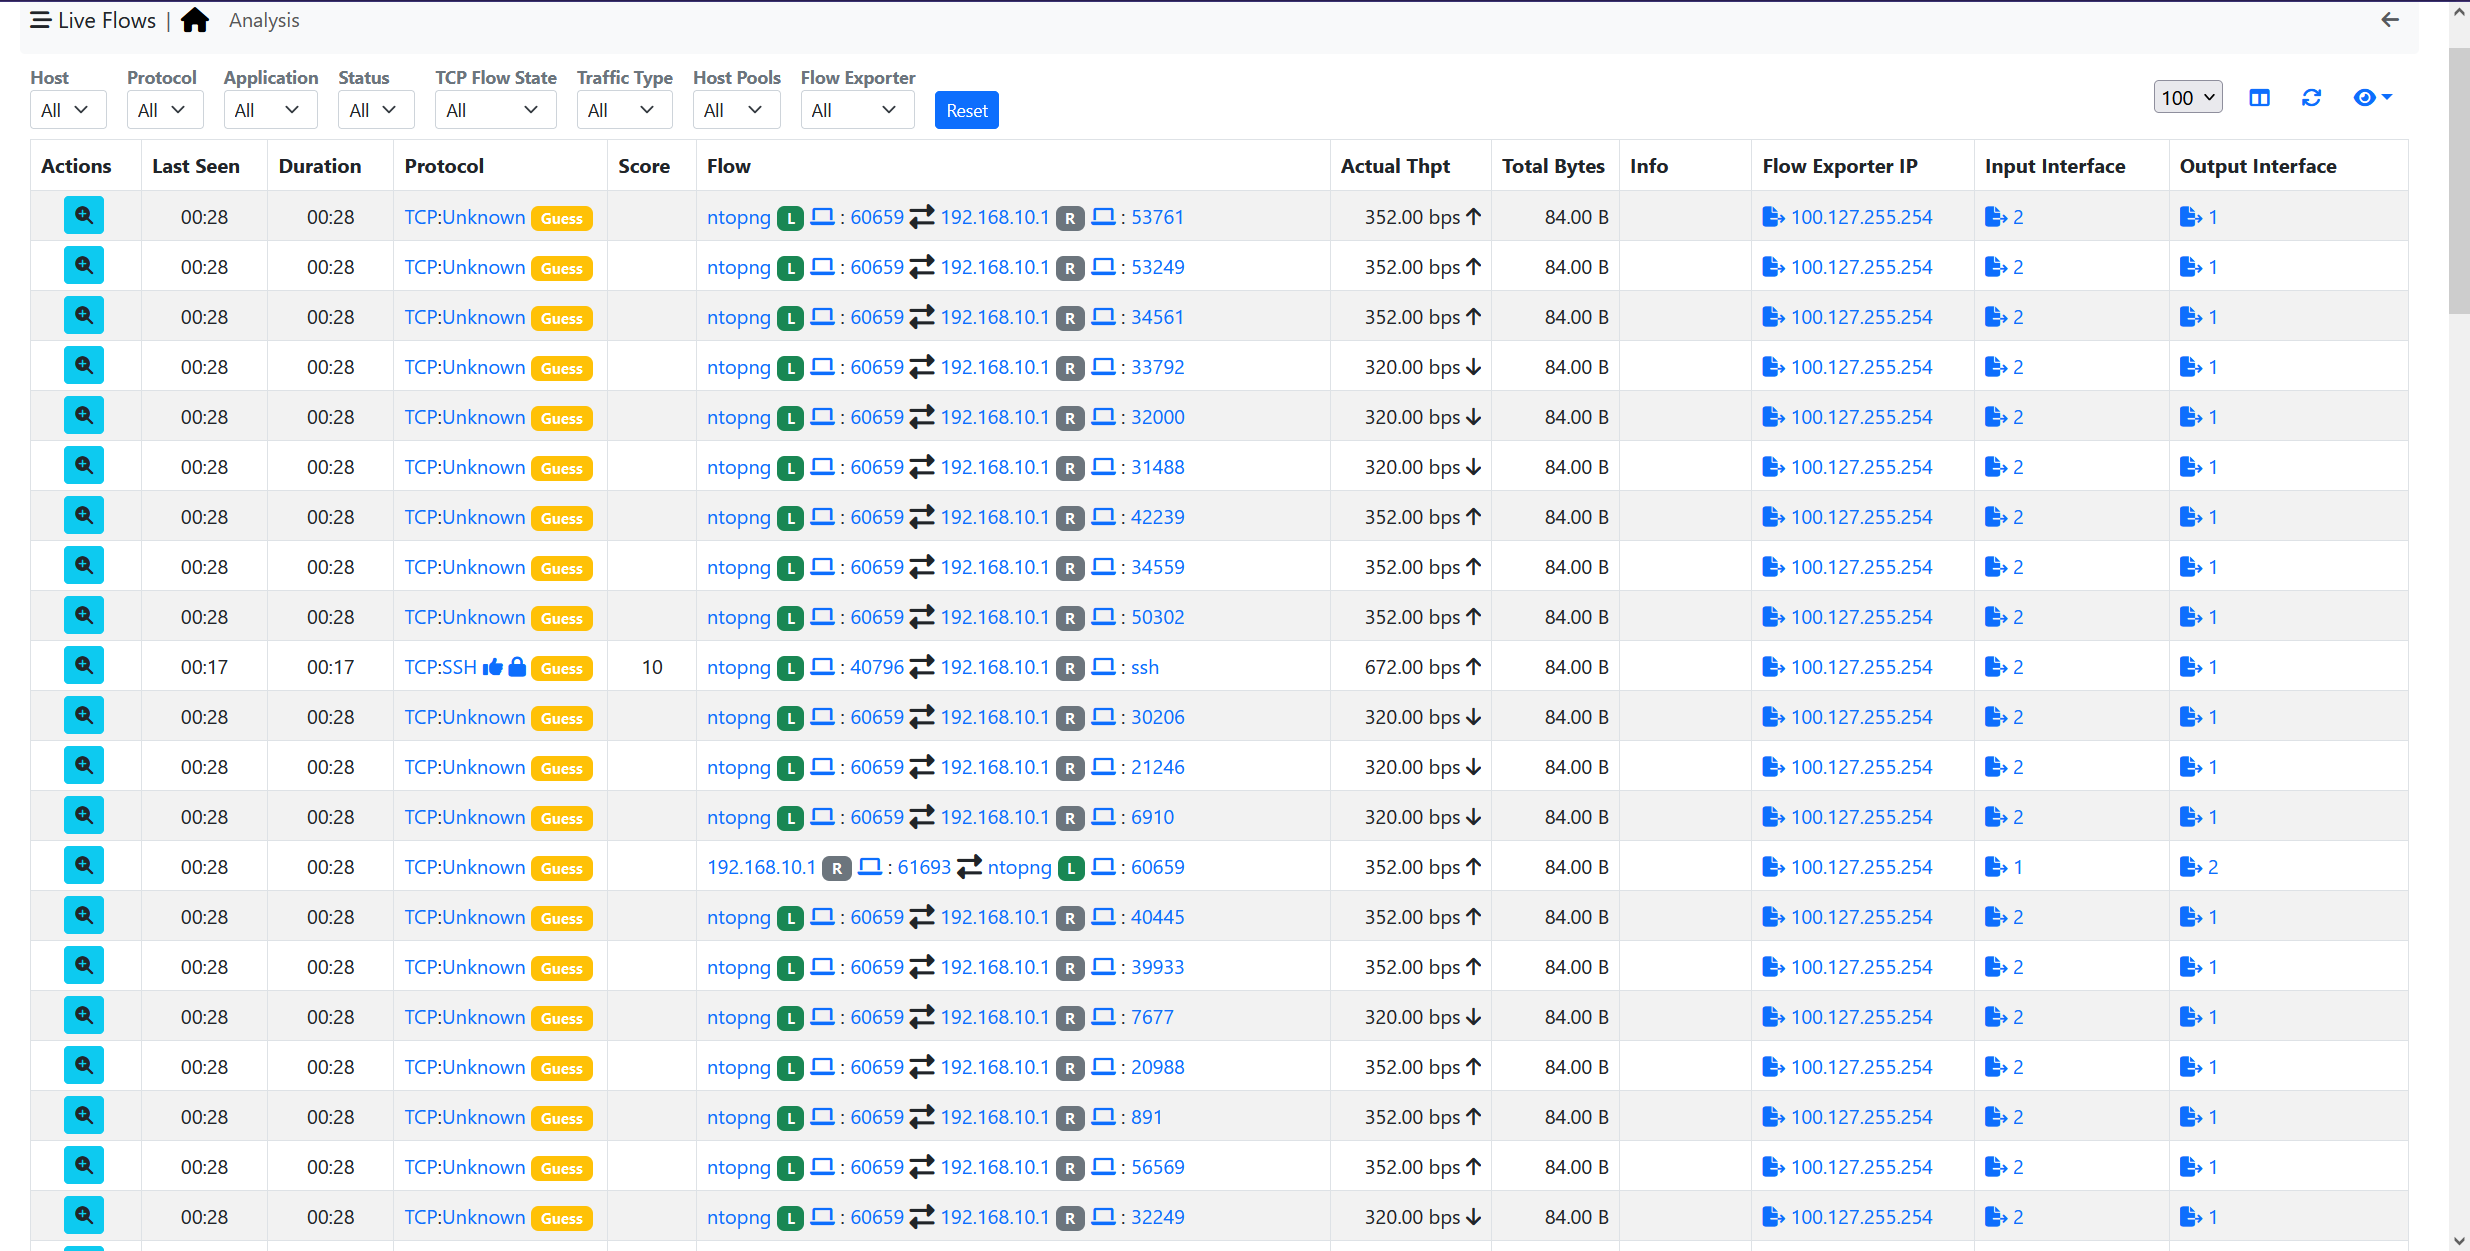
\includegraphics[width=\textwidth]{graphics/nmap_scan_flows.PNG}
    \caption[ntopng met toekomende flows]{elaborate description}
    \label{fig:ntopngFlows}
\end{figure}

\subsection{Overzicht alerts}
Tot slot is het nu ntopng die zorgt voor de beoogde behavioural checks. Hier concludeert hij met hoge severity (100) dat er vanop de server waarop ntopng draait, scanning-activiteit gaande is. In de beschrijving geeft hij bovendien aan waarom hij hiervan uitgaat: 226 scan attempts gedetecteerd, wat ruim boven het verwachtte maximum van 32 ligt.

\begin{figure}[htb]
    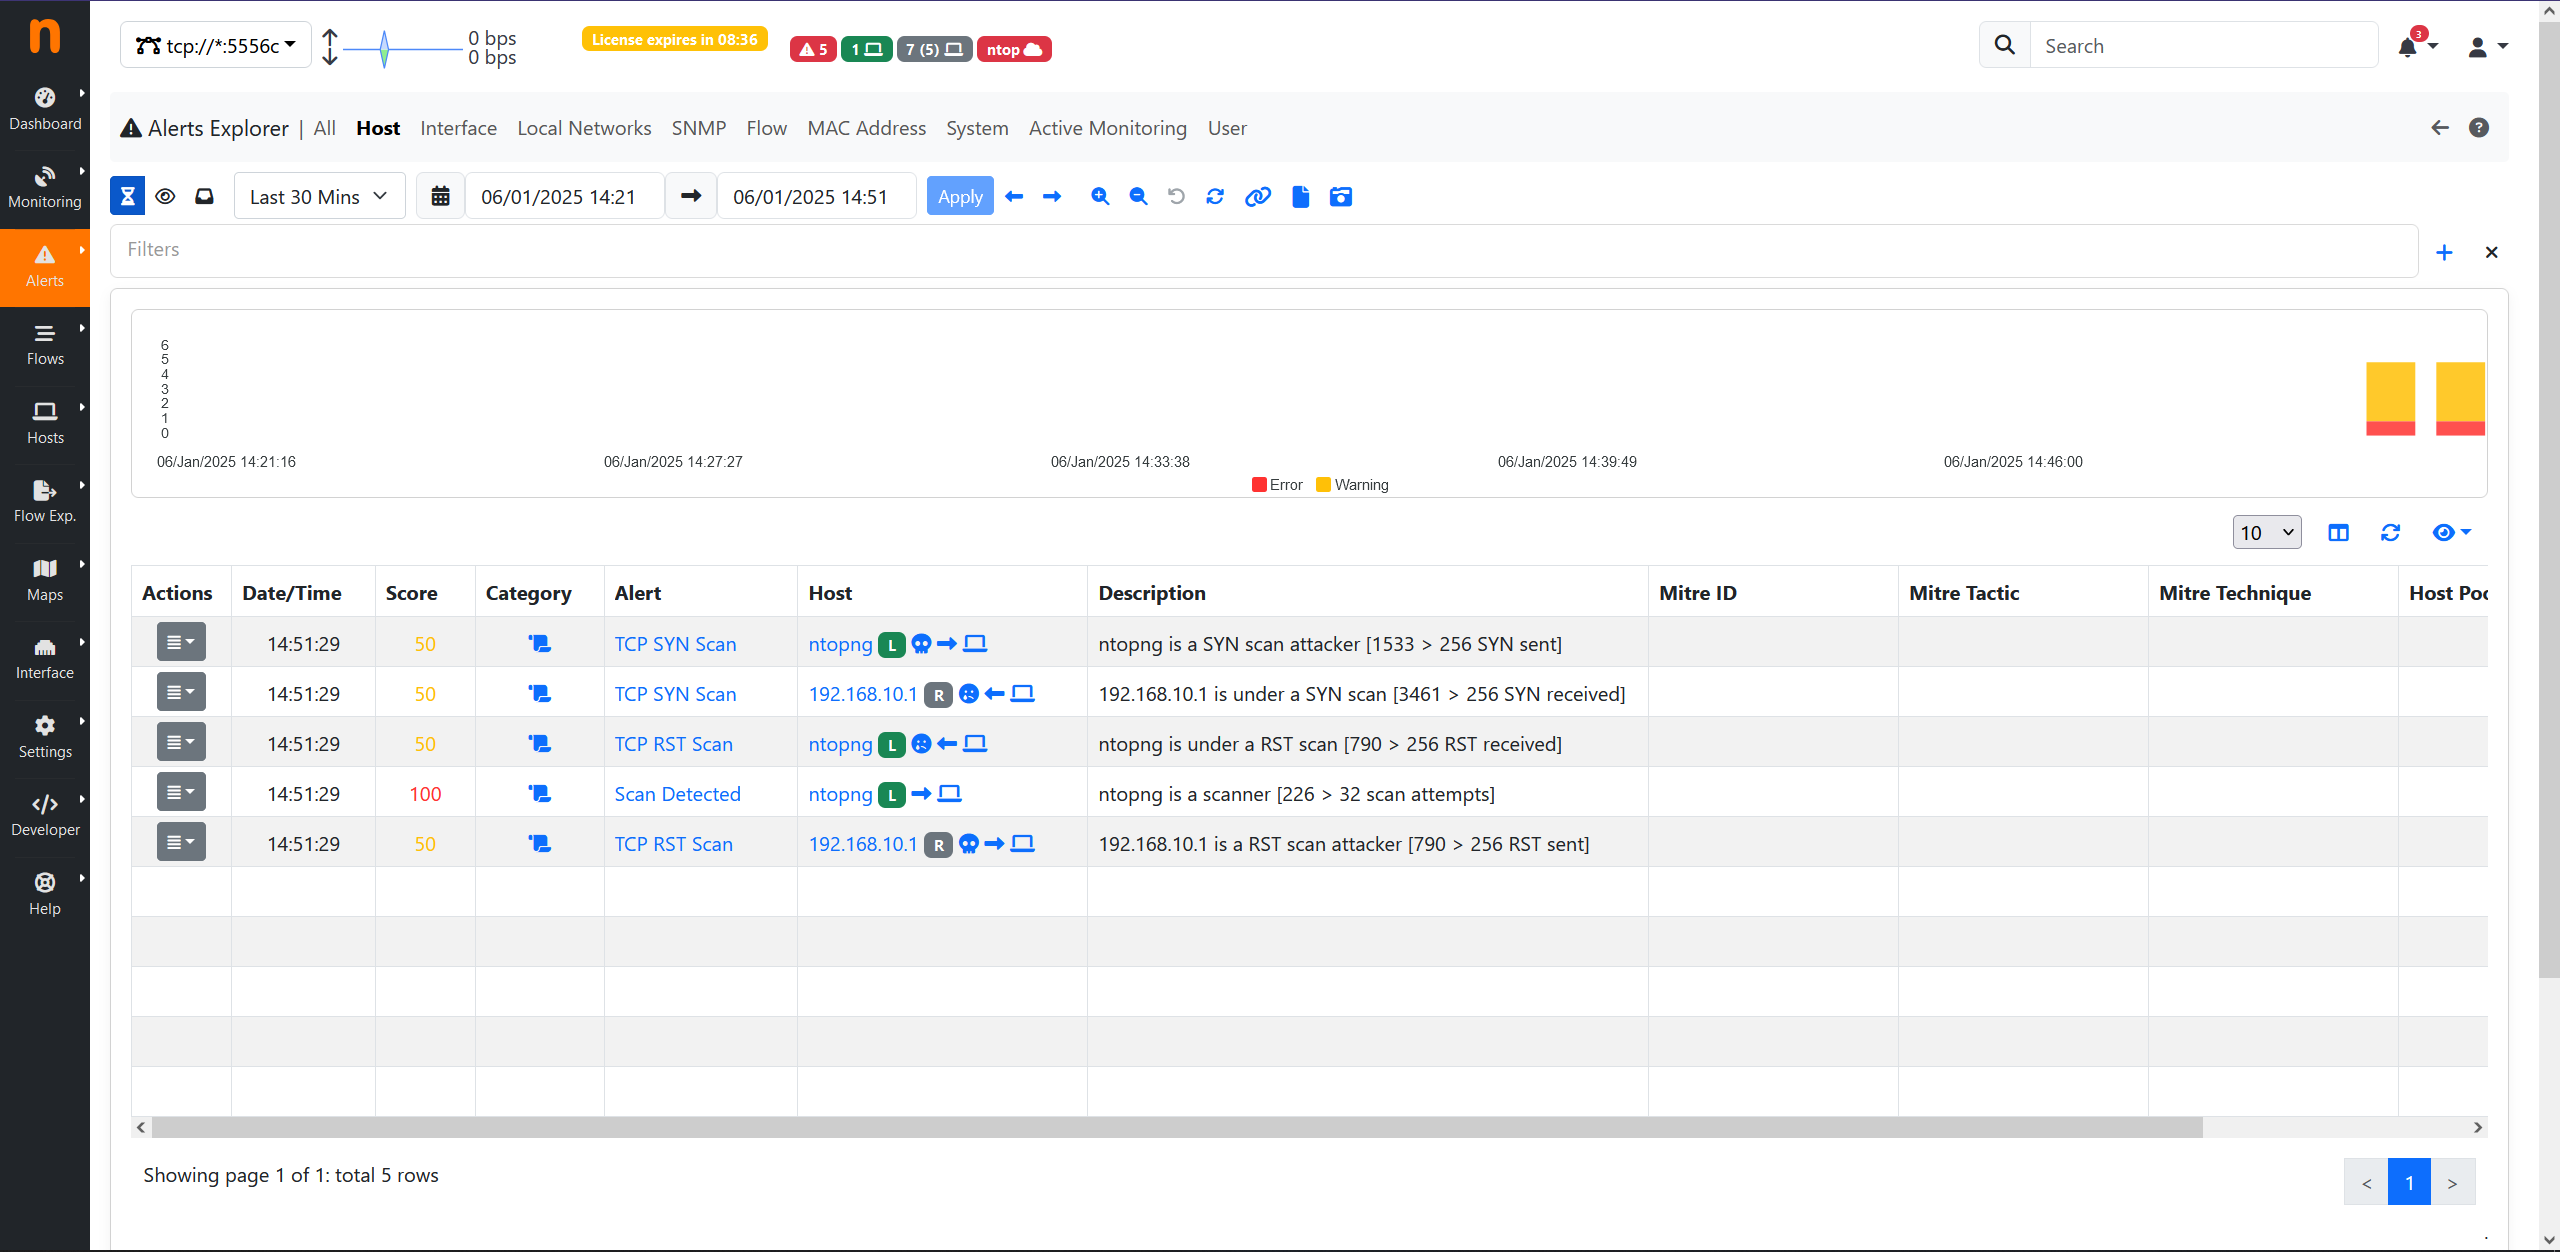
\includegraphics[width=\textwidth]{graphics/nmap_scan.PNG}
    \caption[ntopng scan alerts]{elaborate description}
    \label{fig:ntopngAlerts}
\end{figure}